%*********************************************************************************%
\chapter*{About the author}
\addcontentsline{toc}{chapter}{About the author}
\markboth{About the author}{About the author}

\begin{wrapfigure}{r}{0.3\textwidth}
\centering
\vspace{-4mm}
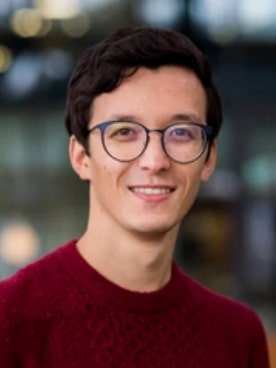
\includegraphics[width=0.3\textwidth]{./fig/Brandon.jpg}
%\caption{This is the caption.}
%\label{test}
\vspace{-9mm}
\end{wrapfigure}
Brandon Caasenbrood was born in Roermond, the Netherlands, on April 29$^{\textrm{th}}$, 1993. After finishing high school in 2011 at the Broekhin college in Roermond, he studied mechanical engineering at the Eindhoven University of Technology (TU/e) in Eindhoven, the Netherlands. In 2016, he did an internship project at the RMIT Melbourne University under the supervision of Liuping Wang focusing on nonlinear Kalman filters for autonomous drones using onboard inertial and ultra-sound sensor measurements. He obtained his BSc and MSc degrees (with honors) at the Eindhoven university in 2014 and 2017, respectively. 

In September 2017, he started as a junior researcher within the Dynamics and Control group at the Department of mechanical engineering of the TU/e. Later, in February 2018, he started his PhD on the topic of design, modeling and control of soft robots under the supervision of Alexander Pogromsky (Sasha) and Henk Nijmeijer. The work focuses on both theoretical and practical aspects related to the design, modeling and control of soft robots. This research is part of the Wearable Robotics perspective program, a Dutch research program funded by the Nederlandse Organisatie voor Wetenschappelijk Onderzoek (NWO). The main results of his research are presented in this dissertation.
%\lipsum*[1-2]